Given a query entity and its known facts, the Ruler leverages rules that describe entities with similar facts to predict facts for the entity in question. Training the ruler means detecting patterns in the training graph structure and storing those patterns in the form of rules. During inference, the Ruler looks for rules whose rule heads apply to the entity in question to predict new facts for it. For performance reasons, inference is implemented as a two-step process, where all rules are processed for all entities together in the first step followed by the individual entity's prediction as a lookup in the second step, but the result is the same. Like the Texter, the Ruler is limited to tail prediction, meaning that it predicts all facts that include the queried entity as the head entity.

For rule mining, AnyBURL, the bottom-up rule mining algorithm, by Christian Melicke et al.~\cite{Meilicke2019AnytimeBR} is used. It is an anytime algorithm, meaning that it can be interrupted anytime and still yield valid results. Bottom-up rule mining refers to the fact that the algorithm starts with concrete paths in the graph and tries to generalize those paths to rules instead of coming up with rules initially and searching for evidence subsequently, which would be a top-down approach. Out of all possible Horn rules that might describe patterns in the graph, AnyBURL is restricted to rules that can be generalized from \emph{ground path rules}. A ground path rule contains only constants - no variables - and must not contain any cycles in its body. The following formula describes a ground path rule of length $n$, meaning that it consists out of the head fact and $n$ body facts:

\begin{align*}
(c_0, h, c_1)
    \Leftarrow (c_1, b_1, c_2), \dots, (c_n, b_n, c_{n+1}) &&
    c_k \neq c_l; k, l \in \{1, \dots, n+1\}, k \ne l
\end{align*}

Notably, despite the rule body being free of cycles, the ground path rule itself might still be cyclic, depending on the rule head. Ground path rules are derived directly from randomly sampled paths in the graph and are subsequently generalized to rules that replace some of the constants with variables. General rules for which further supporting paths can be found are then kept. In the AnyBURL paper, Melicke et al. show that any rule that can be generalized from a ground path rules can be generalized to one of the three rule types formulated in~\ref{eq:4_approach/2_ruler/ac1}~--~\ref{eq:4_approach/2_ruler/c}. $C$ rules can only be generalized from cyclic ground path rules, while $AC1$ and $AC2$ rules can also be generalized from acyclic ones.

\begin{align}
    AC1 && (c_0, h, X) &\Leftarrow (X, b_1, A_2), \dots, (A_n, b_n, c_{n+1})
    \label{eq:4_approach/2_ruler/ac1} \\

    AC2 && (c_0, h, X) &\Leftarrow (X, b_1, A_2), \dots, (A_n, b_n, A_{n+1})
    \label{eq:4_approach/2_ruler/ac2} \\

    C   && (Y, h, X)   &\Leftarrow (X, b_1, A_2), \dots, (A_n, b_n, Y)
    \label{eq:4_approach/2_ruler/c}
\end{align}

At its core, the algorithm repeatedly samples random paths from the graphs, generalizes them to all possible rule types, looks for further paths that match the gained rules, and keeps those rules that fulfill a minimum quality criterion. For example, regarding the simple knowledge graph in~\ref{figure:example_knowledge_graph} that is similar to the one from the AnyBURL paper and assuming that the algorithm has already proceeded to search for rules of length two, AnyBURL might randomly sample the two paths~\ref{eq:4_approach/2_ruler/path_1} and~\ref{eq:4_approach/2_ruler/path_2}.

\begin{figure}[t]
    \centering
    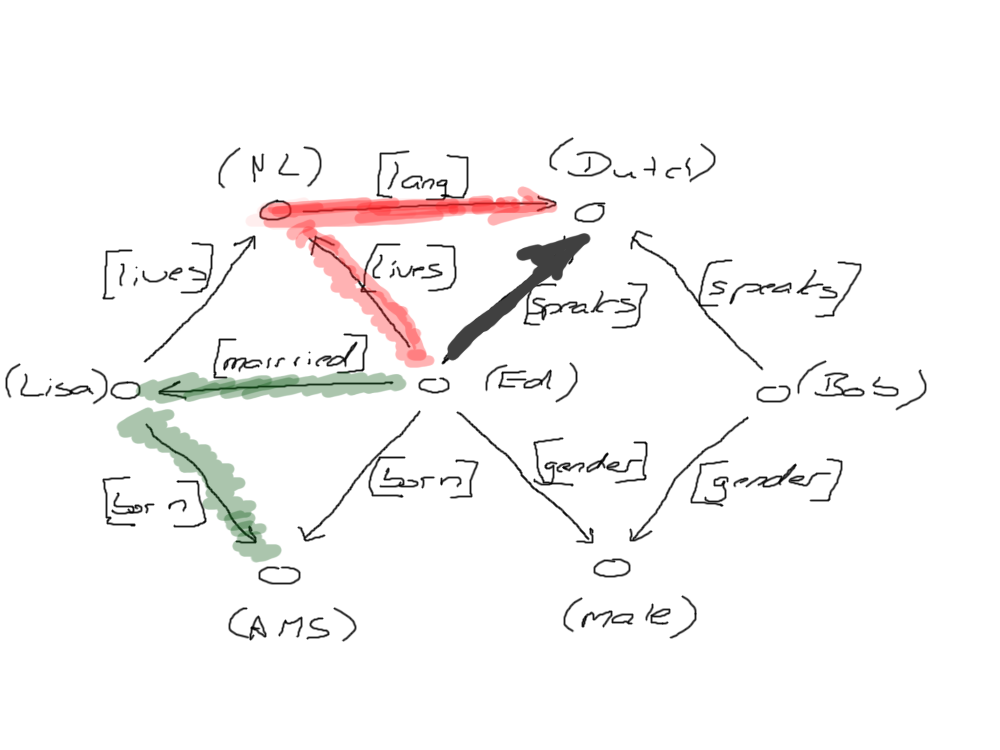
\includegraphics[width=\textwidth]{4_approach/2_ruler/example_knowledge_graph}
    \caption{Modified version of example knowledge graph from AnyBURL paper highlighting a cyclic and an acyclic path}
    \label{figure:example_knowledge_graph}
\end{figure}

\begin{align}
(Dutch)
    \leftarrow [speaks] - (Ed) - [married~to] \rightarrow (Lisa) - [born~in] \rightarrow (AMS)
    \label{eq:4_approach/2_ruler/path_1} \\

    (Dutch) \leftarrow [speaks] - (Ed) - [lives~in] \rightarrow (NL) - [has lang] \rightarrow (Dutch)
    \label{eq:4_approach/2_ruler/path_2}
\end{align}

From those paths, it then derives the ground path rules~\ref{eq:4_approach/2_ruler/ground_path_rule_1} and~\ref{eq:4_approach/2_ruler/ground_path_rule_2} by taking the path's first part as the rule's head and the remaining parts to form the rule body. The direction of relations is thereby ignored.

\begin{align}
(Ed, speaks, Dutch)
    &\Leftarrow (Ed, married~to, Lisa), (Lisa, born~in, AMS)
    \label{eq:4_approach/2_ruler/ground_path_rule_1} \\

    (Ed, speaks, Dutch) &\Leftarrow (Ed, lives~in, NL), (NL, has~lang, Dutch)
    \label{eq:4_approach/2_ruler/ground_path_rule_2}
\end{align}

The acyclic ground path rule~\ref{eq:4_approach/2_ruler/ground_path_rule_1} can be generalized to the $AC1$ rule~\ref{eq:4_approach/2_ruler/rule_1} and the $AC2$ rule~\ref{eq:4_approach/2_ruler/rule_2} while the cyclic ground path rule~\ref{eq:4_approach/2_ruler/ground_path_rule_2} can be generalized to rules~\ref{eq:4_approach/2_ruler/rule_3}~--~\ref{eq:4_approach/2_ruler/rule_5}, covering all three rule types.

\begin{align}
    AC1 && (X, speaks, Dutch) &\Leftarrow (X, married~to, A_2), (A_2, born~in, AMS)
    \label{eq:4_approach/2_ruler/rule_1} \\

    AC2 && (X, speaks, Dutch) &\Leftarrow (X, married~to, A_2), (A_2, born~in, A_3)
    \label{eq:4_approach/2_ruler/rule_2} \\

    AC1 && (X, speaks, Dutch) &\Leftarrow (X, lives~in, A_2), (A_2, has~lang, Dutch)
    \label{eq:4_approach/2_ruler/rule_3} \\

    AC2 && (Ed, speaks, Y) &\Leftarrow (Ed, lives~in, A_2), (A_2, has~lang, Y)
    \label{eq:4_approach/2_ruler/rule_4} \\

    C   && (X, speaks, Y) &\Leftarrow (X, lives~in, A_2), (A_2, has~lang, Y)
    \label{eq:4_approach/2_ruler/rule_5}
\end{align}

Next, every rule candidate is scored by looking for further rule groundings that fulfill the rule body and counting how often the rule head holds. The number of rule groundings that also fulfill the rule body is called the rule's \emph{support}. Together with the ratio of head fulfilling groundings to support, called confidence, the support is usually crucial to the subsequently applied quality criterion that decides whether to keep the rule. It is noteworthy that, although some rules are more general than others, like~\ref{eq:4_approach/2_ruler/rule_2} compared to~\ref{eq:4_approach/2_ruler/rule_1}, the latter are still kept as they might end up with higher confidence for the specific case they cover during the ongoing mining process.

The core process described by the above example is repeated until only a few new rules of the same length can be found. AnyBURL then continues its search for rules of increased length until it terminates after a fixed number of time steps. Listing~\ref{code:anyburl} shows the slightly adjusted pseudocode from the AnyBURL paper. The sampling and scoring process discussed above is implemented as the body of the inner while loop. The outer for loop implements the repeated check for the saturation of rules of the current length and the eventual proceeding to rules of increased length.

A walk through the pseudocode reads as follows: Given the Graph $G$, the saturation threshold $s$, the quality criterion $Q$, a number of iterations $i$ and the timespan $ts$ each iteration endures, AnyBURL starts with an empty ruleset $R$, that will be extended after each iteration and returned in the end. The initial length of the randomly sampled paths is $n=2$, allowing to find the shortest possible rules of length 1. During the first iteration of duration $ts$, AnyBURL fills therule set $R_s$, that keeps the rules found in the current iteration, by repeatedly sampling paths, generating rules from the paths, scoring the resulting rules, and keeping those that fulfill the specified quality criterion. The default quality criterion is rather benevolent, filtering out rules with a support of one and confidence less than 0.0001~\cite{AnyBURL}. At the end of the iteration, when the timespan $ts$ has passed, $R_s^{'}$ is calculated as the set of rules mined during the iteration that were already known. If the share of already known rules mined during the current iteration exceeds the saturation threshold, the algorithm starts searching for rules of increased length, otherwise, it continues with the current length. In both cases, the iteration's rules are added to the overall ruleset $R$. If the specified number of total iterations is reached, AnyBURL terminates and returns the mined rules $R$. In practice, AnyBURL saves the mined rules in a text file at the end and at configurable points during mining.

\begin{listing}
    \begin{lstlisting}
        AnyBURL(G, sat, Q, i, ts):
            n = 2
            R = $\emptyset$
            for i times:
                $R_s = \emptyset$
                start = current_time()
                while current_time() < start + ts:
                    p = sample_path(G, n)
                    $R_p$ = generate_rules(p)
                    for $r$ in $R_p$:
                        score($r$)
                        if $Q$($r)$:
                            $R_s$ = $R_s \cup r$

                $R_s^{'}$ = $R_s \cap R$
                if $|R_s^{'}| / |R_s| > sat$:
                    n = n + 1
                $R$ = $R_s \cup R$

            return $R$
    \end{lstlisting}
    \caption{AnyBURL Rule Mining Algorithm}
    \label{code:anyburl}
\end{listing}

With the stored rules from AnyBURL in place, the Ruler is prepared for inference. Conceptually, given an entity and its known facts, the Ruler loads the rules, filters out bad ones, applies the remaining ones to all known facts, keeps track of the rules that predict facts considering the query entity, and finally ranks all retrieved facts by confidence. The known facts provided with the query entity as well as all facts from the training set are filtered out during the process. For open-world entities, this implies an empty result set as no rule can cover an entity that is not connected to any other entity and all the facts predicted for the train entities will be filtered out.

In more detail, the Ruler initially filters out a large amount of the mined rules by cutting off rules with confidence below 0.5 by default. The remaining rules are \emph{grounded}, in the set of known facts, i.e. ground path rules are searched for the rules. Besides the known facts that come with the query entity, those known facts also include the training facts, because the body of a rule of length $n > 1$ can begin beyond the entities directly connected to the query entity. Next, the Ruler removes rules whose implied fact has a head entity different from the query entity. Finally, besides filtering out already known facts, the remaining facts are sorted by confidence whereby facts predicted by multiple rules are assigned the highest confidence of any of those rules. For convenience, each fact's rules are sorted by confidence as well.
